\chapter{Overview}
\label{chap:overview}

With the growing size of the modern computer software systems, the number of
errors present in such systems has increased.  Moreover, with increasing size
of the code base, the possibility of finding bugs, both manually and
automatically, is decreasing very rapidly. On the other hand, increasing
reliance on computers and computer software systems in every aspect of human
life implies a strong need for reliable software systems.

Software updates are an integral part of the software maintenance process, but
unfortunately present a high risk, with many users and administrators refusing
to upgrade their software and relying instead on outdated versions, which often
leaves them and their systems exposed to software bugs and security
vulnerabilities.

The Hearbleed bug~\cite{heartbleed} is a prime example of this behaviour. A
fixed version of OpenSSL was released on the same day the Heartbleed bug was
publicly disclosed.  However, a month after the publication, despite the wide
media coverage, 1.5\% (12,043) of the 800,000 most popular sites in the world
were still using the vulnerable version of OpenSSL, making their servers
susceptible to attacks~\cite{heartbleed-prevalent}.

Nowadays, many services including large-scale ones such as Google, Facebook or
Amazon employ \emph{continuous deployment}, whereby new versions are
continuously released to users~\cite{johnson2009}. Multiple versions can be
released throughout the day, and each version is often accessible only to a
fraction of users to prevent complete outage in case of an error caused by one
of the new versions.

While this approach helps minimize the number of users affected by newly
introduced bugs, it is not foolproof---bugs introduced by new releases may
manifest themselves only in particular cases or following prolonged operation,
after the release has been deployed to the entire user base. Errors and
failures affecting the majority of the user-base therefore occur even in these
applications. Such outages might cause significant financial losses and
frustration among users, and it is therefore critical to avoid them.

An example of such disruption is the recent Verizon
outage~\cite{verizon-outage2014} of the billing and activation system,
affecting a large number of users which were unable to log into their accounts.
After the incident, Verizon issued the following statement:
\begin{quotation}
The Verizon Wireless billing system was fully restored early today, shortly
after midnight. The issue affecting some customer access to account information
was an unintended consequence of a software update performed by the company on
its billing system two days ago.
\end{quotation}
The outage, which according to reports lasted for 48 hours, was so impactful
that it generated a lot of negative reactions from frustrated customers
including its own \textsf{\#verizonfail} and \textsf{\#verizonoutage} Twitter
hashtags.  This as well as other similar incidents (\eg
Blogger~\cite{blogger-incident2011} or Facebook~\cite{facebook-incident2010})
show the possible consequences of failed software updates.

The problems caused by failed software updates are also not restricted to
server applications or services. \vim,\footnote{\url{http://www.vim.org/}}
arguably one of the most popular text editors, shipped with the popular
Ubuntu Linux distribution has been also affected by failed software updates in
the past.  In version 7.1.127, while trying to fix a memory leak, \vim
developers introduced a double \textstt{free} bug that caused \vim to crash
whenever the user tried to use a path completion feature.  This bug made its
way into Ubuntu 8.04, affecting a large number of
users.\footnote{\url{https://bugs.launchpad.net/ubuntu/+source/vim/+bug/219546}}

\section{Problem statement}
\label{overview:problem}

Software updates pose an important problem. We aim to tackle this problem using
a simple yet effective \emph{multi-version execution} approach: instead of
running only of the software versions, we run multiple versions in parallel; by
carefully coordinating their executions and selecting the behaviour of the more
reliable version when they diverge, we create a more secure and dependable
multi-version application.

\begin{figure}[t]
  \begin{subfigure}[b]{0.5\textwidth}
    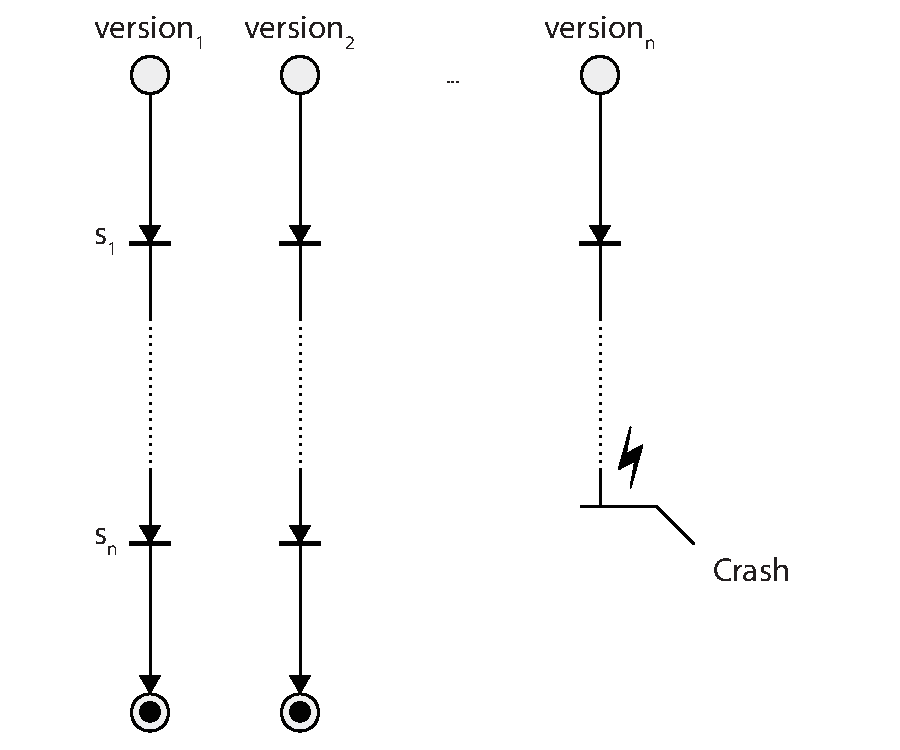
\includegraphics[width=\textwidth]{overview/figures/failover}
    \caption{Failover scheme.}
    \label{fig:failover-scheme}
  \end{subfigure}
  \quad
  \begin{subfigure}[b]{0.5\textwidth}
    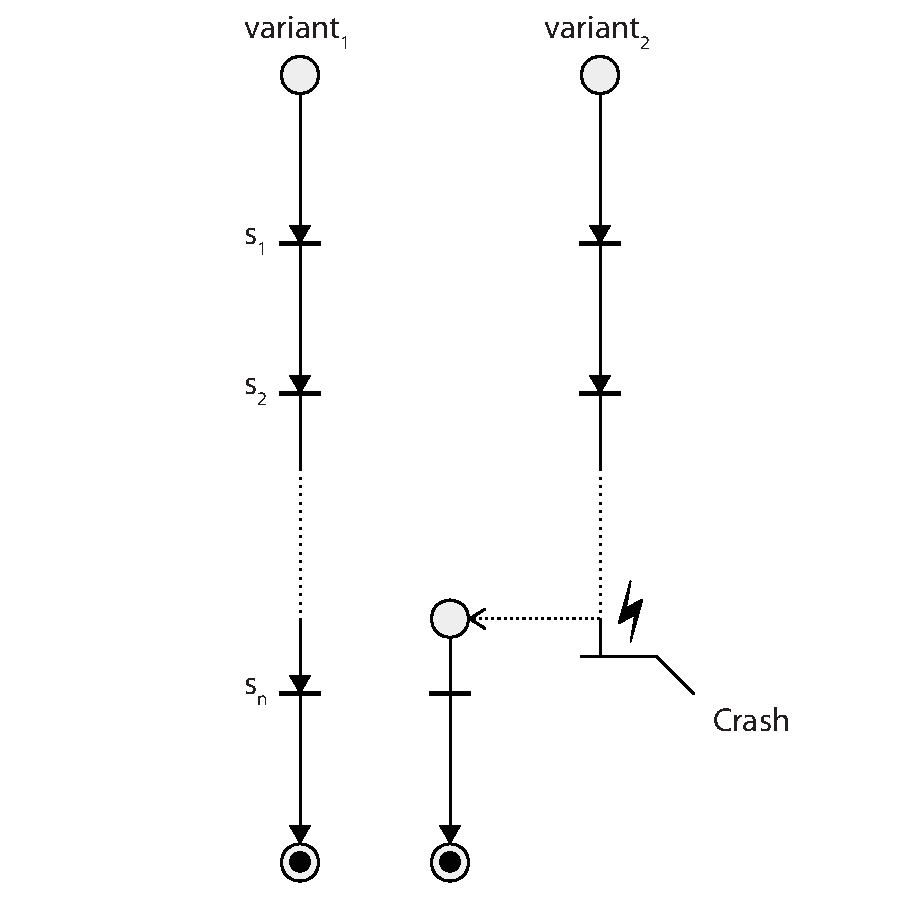
\includegraphics[width=\textwidth]{overview/figures/failrecovery}
    \caption{Failure recovery scheme.}
    \label{fig:failrecovery-scheme}
  \end{subfigure}
  \caption{Two schemes of multi-version execution presented in the thesis.}
  \label{fig:mvx-schemes}
\end{figure}

In this thesis, we present two different schemes for implementing the
multi-version execution technique. The first is the failover scheme, shown in
Figure~\ref{fig:failover-scheme}, in which $N$ different versions are being run
in parallel, and if one these versions fail, we transparently switch to other
one. This scheme offers minimal performance overhead enabling the use of large
number of versions, but offers only limited guarantees in case of failure.  In
addition, we propose a failure recovery scheme, conceptually depicted in
Figure~\ref{fig:failrecovery-scheme}, which allows program to survive errors
introduced by software patches. However, as a trade-off, this scheme introduces
a larger perfomance penalty and is limited to only two versions being run in
parallel.

% To tackle the software update problem, we propose \emph{multi-version
% execution}, a novel technique, which fits within the overall theme of
% $N$-version programming~\cite{avizienis:nvp,chen1995}. The goal of this
% technique is to improve the software update process to increase software
% availability and reliability by exploiting the abundance of resources (\eg idle
% processor time) made available by modern highly parallel platforms. Whenever a
% new system update becomes available, instead of upgrading the software to the
% newest version, we run the new version in parallel with the old one; by
% carefully coordinating their executions and selecting the behaviour of the more
% reliable version when they diverge, we create a more secure and dependable
% multi-version application. As new versions arrive, we continue to execute them
% in parallel with the existing ones, until all available resources have been
% exhausted, or a user-specified threshold has been reached.  At that point, we
% can either discard the very oldest versions, or we can use more sophisticated
% replacement strategies.

The multi-version execution technique fits within the overall theme of
$N$-version programming~\cite{avizienis:nvp,chen1995}. The goal of this
technique is to improve the software update process to increase software
availability and reliability by exploiting the abundance of resources (\eg idle
processor time) made available by modern highly parallel platforms.  We believe
that multi-version execution updates is a timely solution in the context of
today's computing platforms~\cite{multiplicity}. The last decade has seen the
emergence of new hardware platforms, ranging from multi-core processors to
large-scale data centers, which provide an abundance of computational resources
and a high degree of parallelism. These platforms already benefit applications
with a great amount of inherent concurrency.  However, there has been
relatively little progress in exploiting this abundance of resources to improve
software reliability and availability, especially in the context of software
updates.

Typical data centres are designed for peak load to ensure service-level
agreements are met. Servers are rarely completely idle but they do not operate
near their maximum utilisation; most of the time, they operate at between 10\%
and 50\% of their maximum utilization levels. However, even an energy-efficient
server consumes half its full power when doing virtually no work---and for
normal servers, this ratio is much worse~\cite{barroso2007}.  Therefore,
instead of dynamically switching off unused servers which is not effective, we
aim to use the abundance of these resources (\ie processing power) to increase
software availability and reliability.

Our approach aims to improve the reliability of the software update process by
taking advantage of idle resources---such as idle cores on a CPU and idle
servers in a data center---to run multiple versions of an application in
parallel, with the goal of improving the overall reliability and security of
the software being upgraded.  Our current focus is on multi-core processors,
but we believe this solution could be adapted to work on other parallel
platforms as well.  Furthermore, this update mechanism could be extended to
work with a large number of versions running in parallel and configured to
balance conflicting requirements such as performance, reliability and energy
consumption.

There are three main challenges that we need to address to make this approach
viable. First, we need to implement mechanisms for effectively coordinating the
parallel execution of multiple program versions.  Second, when executions
diverge, we need to select the output of the more reliable one, and potentially
merge them back once executions converge again.  Finally, we need to ensure
that the overall system is able to scale up and down the number of program
versions run in parallel in order to balance conflicting requirements such as
performance, reliability, and energy consumption.

%%%%%%%%%%%%%%%%%%%%%%%%%%%%%%%%%%%%%%%%%%%%%%%%%%%%%%%%%%%%%%%%%%%%%%%%%%%%

%We aim to tackle this problem using a simple but effective approach based on
%application-level virtualization.  Whenever a new program update becomes
%available, instead of upgrading the software to the newest version, we {\it
%run the new version in parallel with the old}.  As new versions arrive, we
%continue to execute them in parallel with the existing ones, until all
%available resources have been exhausted, or a user-specified threshold has
%been reached.  At that point, we can either discard the very oldest versions,
%or we can use more sophisticated replacement strategies.  This approach can
%be extended to work with a large number of versions run in parallel, and can
%be applied to several different platforms, ranging from multicore processors
%to large-scale data centers.  

%The rest of this paper is organized as follows. Section~\ref{sec:background}
%discusses related work and  Section~\ref{sec:motivation} motivates our
%approach by using a scenarios based on Google Chrome web browser and Vim text
%editor.  Then, Section~\ref{sec:challenges} discusses the main challenges that
%we need to address to make this approach work in practice and
%Section~\ref{sec:prototype} presents a protype implementing safe updates
%in the context of multi-core processors. Finally, Section~\ref{sec:opportunities}
%describes the potential future work and Section~\ref{sec:conclusion} concludes.

%The rest of this paper is organized as follows. Section~\ref{sec:background}
%discusses related work and  Section~\ref{sec:motivation} motivates our
%approach by using a scenarios based on Google Chrome web browser and Vim text
%editor.  Then, Section~\ref{sec:challenges} discusses the main challenges that
%we need to address to make this approach work in practice and
%Section~\ref{sec:prototype} presents a protype implementing safe updates
%in the context of multi-core processors while Section~\ref{sec:evaluation}
%shows a case study for our approach. Finally, Section~\ref{sec:opportunities}
%describes future work and Section~\ref{sec:conclusion} concludes.

%% Following work presents our approach approach, its advantages and
%% disadvantages. Furthermore, it provides comparison and summarizes
%% differences from the existing solutions aiming to achieve similar
%% goals.



\section{Organisation}
\label{overview:organisation}

The rest of the thesis is organized as follows:

\begin{chapterdescription}
\item[Chapter~\ref{chap:multi-version}] gives an overview of the $N$-version,
  multi-variant and multi-version execution techniques and sets the background
  for the rest of the thesis. The chapter also presents several real-world
  scenarios which are used throughout the thesis as a part of the evaluation.

\item[Chapter~\ref{chap:evolution}] presents a study of software evolution in
  several real-world open-source systems and acts as a motivation for many of
  the design choices made in the systems presented in this thesis.

\item[Chapter~\ref{chap:efficient-execution}] describes \varan, an efficient
  $N$-version monitor designed to run a: large number of versions in parallel.
  The chapter presents the high-level architecture as well as details of the
  prototype implementation, and includes a thorough evaluation including a
  comparison with previous systems.

\item[Chapter~\ref{chap:safe-updates}] presents \mx, a multi-version execution
  runtime focused on fail-recovery from crashes caused by bugs introduced in
  software updates. The chapter gives a detailed overview of the fail-recovery
  mechanism and explains how \mx survives bugs in several existing open-source
  applications.

\item[Chapter~\ref{chap:applications}] introduces other possible applications
  of multi-version and $N$-version execution techniques, such as live
  sanitization, record and replay and security honeypots.

\item[Chapter~\ref{chap:related}] discusses work related to $N$-version and
  multi-version execution both in the reliability and the security context.
\end{chapterdescription}

Finally, the thesis concludes with Chapter~\ref{chap:conclusion}, which
summarizes the contributions, discusses the possible future work and raises
additional research questions.

%The rest of this paper is structured as follows.
%Section~\ref{sec:overview} gives a high-level overview of our
%approach, while Section~\ref{sec:prototype} presents our prototype
%implementation in detail.  Then, Section~\ref{sec:evaluation}
%evaluates our prototype on a set of micro- and macro-benchmarks,
%Section~\ref{sec:applications} shows the applicability to different
%application scenarios, and Section~\ref{sec:discussion} discusses the
%main implications of our design.  Finally, Section~\ref{sec:related}
%presents related work and Section~\ref{sec:conclusion} concludes.

\section{List of publications}
\label{overview:publications}

The text of this thesis is based on, and borrows heavily from the work and the
writing in the following papers:

\begin{itemize}
\item \fullcite{mvupdates12}
\item \fullcite{mx}
\item \fullcite{covrig:issta14}
\item \fullcite{varan:asplos15}
\end{itemize}

